\chapter{Transcript of Stakeholder Feedback Interviews}
\label{app:stakeholder_feedback_interviews}
\addcontentsline{toc}{chapter}{Transcript of Stakeholder Feedback Interviews}

\hspace*{\parindent}The following statements were given by SK Chairpersons after being shown the KABISIG system during the development phase.
\vspace{5mm}

\subsection*{Figure 1. Resolution Management}

\begin{center}
    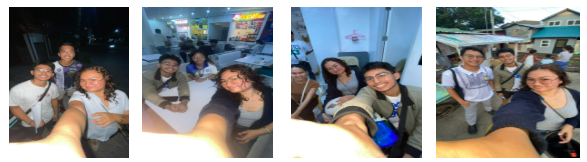
\includegraphics[width=0.75\textwidth]{figures/1.png}
    \par\smallskip
    Resolution Management Screenshot
\end{center}

\noindent
\textbf{Statement 1 by SK Chairperson of TABUCO, BALATAS, CONCEPCION GRANDE, DAYANGDANG:}

\hspace*{\parindent}"The resolution tracking feature is very helpful. Before, we had to write resolutions in Word, print them, and it was difficult to track whether they had already been approved. The youth also had no knowledge of our resolutions. With KABISIG, everyone can see the status of resolutions and participate in youth polls and voting on council matters. This is a great help in making the SK more transparent."\vspace{5mm}


\subsection*{Figure 2. KK Profiling}

\begin{center}
    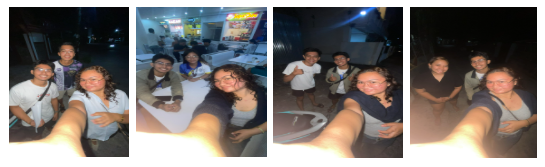
\includegraphics[width=0.75\textwidth]{figures/2.png}
    \par\smallskip
    KK Profiling Screenshot
\end{center}

\noindent
\textbf{Statement 2 by SK Chairperson of BALATAS, CONCEPCION GRANDE, TABUCO, DAYANGDANG, IGUALDAD, SAN FELIPE:}

\hspace*{\parindent}"KK profiling should come first before anything else. We need to know the composition of our youth — students, PWDs, registered voters, unemployed, and scholars. Right now, we simply assume what programs are needed. For example, if we see that there are many unemployed youth, we can immediately create a skills training program. With KABISIG, the demographics are visible right away, so we no longer have to guess what programs are appropriate for our community."\vspace{5mm}


\subsection*{Figure 3. Beneficiary Monitoring}

\begin{center}
    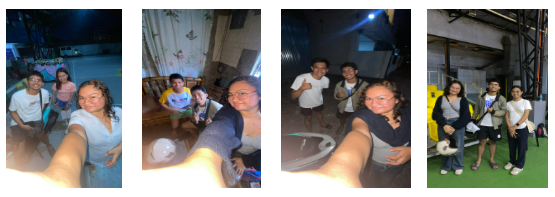
\includegraphics[width=0.75\textwidth]{figures/3.png}
    \par\smallskip
    Beneficiary Monitoring Screenshot
\end{center}

\noindent
\textbf{Statement 3 by SK Chairperson of BALATAS, CONCEPCION GRANDE, TABUCO, DAYANGDANG, CONCEPCION PEQUEÑA:}

\hspace*{\parindent}"Our problem is monitoring who is actually being helped. Some youth receive multiple forms of assistance — educational aid, school supplies, and financial aid — while others receive nothing at all. The SK fails to notice this because there is no system in place. With KABISIG, we can see how many programs each youth has already participated in and who has not yet received any benefit. This effectively prevents duplication of assistance and eliminates favoritism."\vspace{5mm}


\subsection*{Figure 4. Budget Transparency}

\begin{center}
    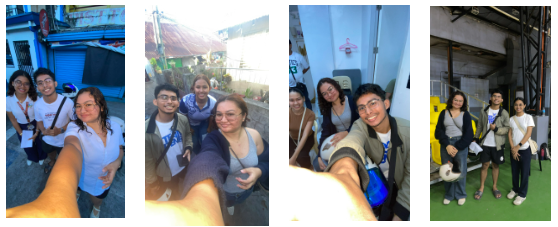
\includegraphics[width=0.75\textwidth]{figures/4.png}
    \par\smallskip
    Budget Transparency Screenshot
\end{center}

\noindent
\textbf{Statement 4 by SK Chairperson of TABUCO, DAYANGDANG, CONCEPCION GRANDE, IGUALDAD, BALATAS:}

\hspace*{\parindent}"The public should be able to see the SK's budget — how much was allocated, how much was spent, and how much remains. For example, if the budget for the Basketball League is ₱35,000, everyone can see that ₱30,000 has already been spent and ₱5,000 is still remaining. This increases transparency and builds the community's trust in the SK. The SK's financial records should be open and accessible to everyone."\vspace{5mm}


\subsection*{Figure 5. Automated Budgeting}

\begin{center}
    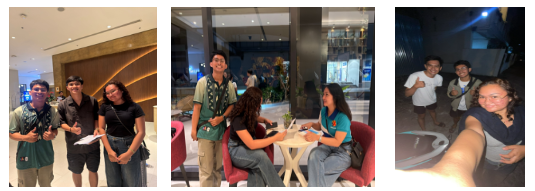
\includegraphics[width=0.75\textwidth]{figures/5.png}
    \par\smallskip
    Automated Budgeting Screenshot
\end{center}

\noindent
\textbf{Statement 5 by SK Chairperson of BALATAS, IGUALDAD, CONCEPCION GRANDE, TABUCO, TINAGO:}

\hspace*{\parindent}"Our treasurer is very pleased because the system already has the formulas built in. She no longer needs to manually compute VAT and non-VAT amounts for every transaction. For example, if we purchase a sound system worth ₱10,000, the system automatically computes the VAT, withholding tax, and net payable amount. Before, we relied on Excel which was time-consuming and prone to errors. Now, our budgeting process is far more accurate and much faster."\vspace{5mm}


\subsection*{Figure 6. Document Management}

\begin{center}
    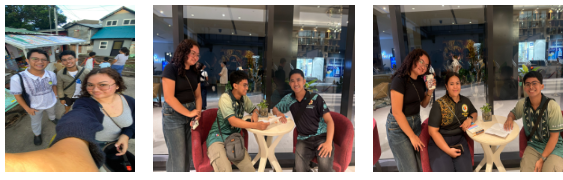
\includegraphics[width=0.75\textwidth]{figures/6.png}
    \par\smallskip
    Document Management Screenshot
\end{center}

\noindent
\textbf{Statement 6 by SK Chairperson of TABUCO, DAYANGDANG, CONCEPCION GRANDE, BALATAS, PANICUASON:}

\hspace*{\parindent}"Our documents used to be completely disorganized — piled up in different folders and scattered across Messenger chats. We did not know whether a voucher had already been approved or whether the liquidation was still pending. With KABISIG, all documents are stored in a single repository — resolutions, budget proposals, vouchers, attendance sheets, accomplishment reports, and photos. The status of each document is immediately visible. No more searching through folders and group chats just to find one file."\vspace{5mm}


\subsection*{Figure 7. Notifications \& Announcements}

\begin{center}
    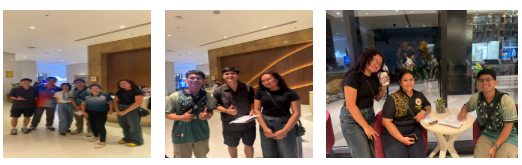
\includegraphics[width=0.75\textwidth]{figures/7.png}
    \par\smallskip
    Notifications \& Announcements Screenshot
\end{center}

\noindent
\textbf{Statement 7 by SK Chairperson of PANICUASON, CALAUAG, TABUCO, SAN FELIPE, CONCEPCION PEQUEÑA:}

\hspace*{\parindent}"The notification system is excellent — it sends automated reminders before, during, and after events. For example, for a Clean-Up Drive scheduled on July 15, the system sends a reminder 7 days before, another 1 day before, a reminder on the event day itself, and a follow-up after the event prompting participants to complete the evaluation form. Youth will no longer forget about activities, and they can also provide feedback afterward. This is a great help in improving youth participation and program accountability."\vspace{5mm}


\subsection*{Figure 8. Inventory Management}

\begin{center}
    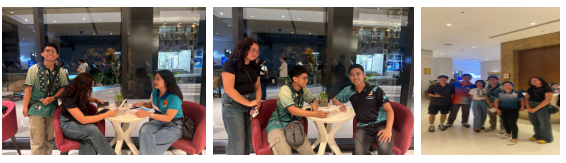
\includegraphics[width=0.75\textwidth]{figures/8.png}
    \par\smallskip
    Inventory Management Screenshot
\end{center}

\noindent
\textbf{Statement 8 by SK Chairperson of TABUCO, BALATAS, CONCEPCION GRANDE, IGUALDAD, LIBOTON:}

\hspace*{\parindent}"We need a system to properly track the SK's assets — tables, chairs, speakers, and other equipment. Before, we would lose track of our inventory, especially during the turnover of officers at the end of each SK term. With KABISIG, all assets and their corresponding quantities are properly recorded in the system. When new SK officials take over, an inventory turnover report is automatically generated. Equipment will no longer go missing, and every official is held accountable for the assets under their care."\vspace{5mm}


\subsection*{Figure 9. Calendar \& Activity Management}

\begin{center}
    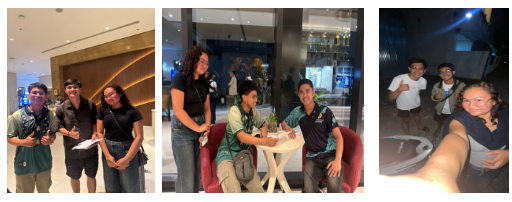
\includegraphics[width=0.75\textwidth]{figures/12.png}
    \par\smallskip
    Calendar \& Activity Management Screenshot
\end{center}

\noindent
\textbf{Statement 9 by SK Chairperson of DAYANGDANG, BALATAS, TABUCO, CONCEPCION GRANDE, CALAUAG:}

\hspace*{\parindent}"We need a calendar view of all SK activities — a monthly overview showing event schedules, assigned officials, locations, and related documents. Before, our schedules would conflict and we were unable to properly monitor our activities. With KABISIG, we can immediately see which projects are upcoming, ongoing, and already completed. There is also a historical record of all SK activities, which is very useful for reporting, evaluation, and planning future programs."\vspace{5mm}